\quest{9.1.6}
Seja $G$ um grafo 2-conexo com pelo menos 4 vértices. Seja $e \in E(G)$ uma
aresta qualquer. Suponha que $e = uv$ não seja contraível. Mostraremos que $e$
é deletável.

Sejam $x, y \in V(G)$, $x \ne y$, dois vértices quaisquer. Sabemos que eles
possuem entre si dois caminhos $P_{xy}$ e $P'_{xy}$ internamente disjuntos. Se
$e$ não pertence a nenhum desses caminhos, em $G \setminus e$ os dois caminhos
continuam existindo e o resultado segue. Além do mais, $e$ não pode pertencer a
$P_{xy}$ e $P'_{xy}$ pois, caso contrário, eles não seriam internamente
disjuntos. Sem perda de generalidade, suponha que $e \in E(P_{xy})$.
Mostraremos que podemos construir dois caminhos internamente disjuntos entre
$x$ e $y$ que não usam a aresta $e$.

Como $G$ é 2-conexo, existem dois caminhos $P_{uy}$ e $P'_{uy}$ entre $u$ e
$y$. Sem perda de generalidade, suponha que o caminho $P'_{uy}$ seja o primeiro
a intersectar o caminho $P'_{xy}$ em um vértice $s$. Sejam $P = xP_{xy}tP_{uy}$
e $P' = xP'_{xy}sP'_{uy}$, tal que $t$ é o último vértice de $P_{uy}$ a
intersectar a porção $xP_{xy}u$ de $P_{xy}$, dois caminhos de $x$ a $y$ (veja
Figura ~\ref{fig:grafoq916}).

\begin{figure}[htb]
    \centering
    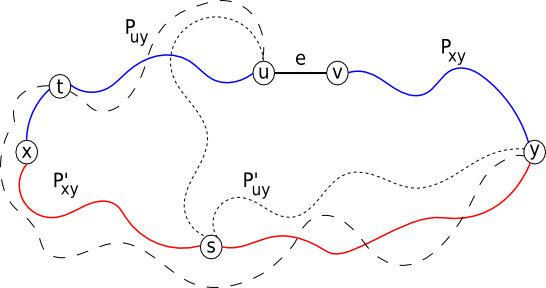
\includegraphics[height=5cm, width=9.4cm]{figuras/graph_q916}
    \caption{A aresta $e$ é deletável.}
    \label{fig:grafoq916}
\end{figure}

Resta mostrar que $P$ e $P'$ são internamente disjuntos.  Para isso, note que
$P_{uy}$ não intersecta a porção $xP'_{xy}s$ pois, por definição, $P'_{uy}$ é o
primeiro a intersectar $P'_{xy}$. Além do mais, sabemos que $P_{uy}$ e
$P'_{uy}$ são internamente disjuntos e portanto, $sP'_{uy}$ e $tP_{uy}$ também
o são. Então, $P$ e $P'$ são dois caminhos entre $x$ e $y$ internamente
disjuntos e que não usam a aresta $e$. Portanto $\kappa(G \setminus e) =
\kappa(G)$ e $e$ é deletável.
\fimprova

